\chapter{Metodologia Científica}

Não pretendemos, neste capítulo, fazer uma discussão complexa do que é o método científico, mas mostrar algumas noções básicas que devem ser pensadas \textbf{antes} de começar o trabalho. 
Partimos, então, de uma visão do método científico que é bastante geral.

\citet{Bunge2002} apresenta uma visão epistemológica da investigação científica como uma sequência de atividades~\citep[p. 39-40]{Bunge2002}\footnote{Tradução livre do autor}:
\begin{quote}
\begin{enumerate}
    \item Descobrimento do Problema ou lacuna em um conjunto de conhecimentos. Se o problema não está enunciado com clareza, se passa à etapa seguinte, se não, à subsequente;
    \item Descrição precisa do problema, se possível em termos matemáticos, mas não necessariamente quantitativos, ou uma nova descrição de um velho problema a luz de novos conhecimentos 
    \item Busca de conhecimentos ou instrumentos relevantes ao problema (por exemplo, dados empíricos, teorias, aparatos de medida, técnica de cálculo ou de medida). Ou seja, inspeção do conhecido para ver se é possível resolver o problema;
    \item Tentativa de solução do problema com ajuda dos meios identificados. Se essa tentativa falha, passasse à etapa seguinte, se não, à subsequente.
    \item Invenção de novas ideias (hipóteses, teorias ou técnicas) ou a produção de novos dados empíricos que prometam resolver o problema;
    \item Obtenção uma solução, exata ou aproximada, do problema com auxílio do instrumental conceitual ou material disponível;
    \item Por a prova a solução, por exemplo, com ensaios de laboratório ou de campo, e
    \item Correções necessárias nas hipóteses ou técnicas, ou mesmo na formulação do problema original.
\end{enumerate}
\end{quote}

Essa descrição, ilustrada na Figura \ref{fig:bunge}, é o que se chama na Engenharia de Software de um processo Linear ou em Cascata, mas é óbvio que isso é só uma abstração que facilita a descrição a nível epistemológico. A pesquisa científica é um processo de aprendizado constante, e muitas vezes é necessário, após uma etapa, voltar atrás, ou pular a frente, de forma a melhorar a compreensão do problema, das soluções possíveis, corrigir experimentos, etc.



\begin{figure}[hbt]
    \centering
	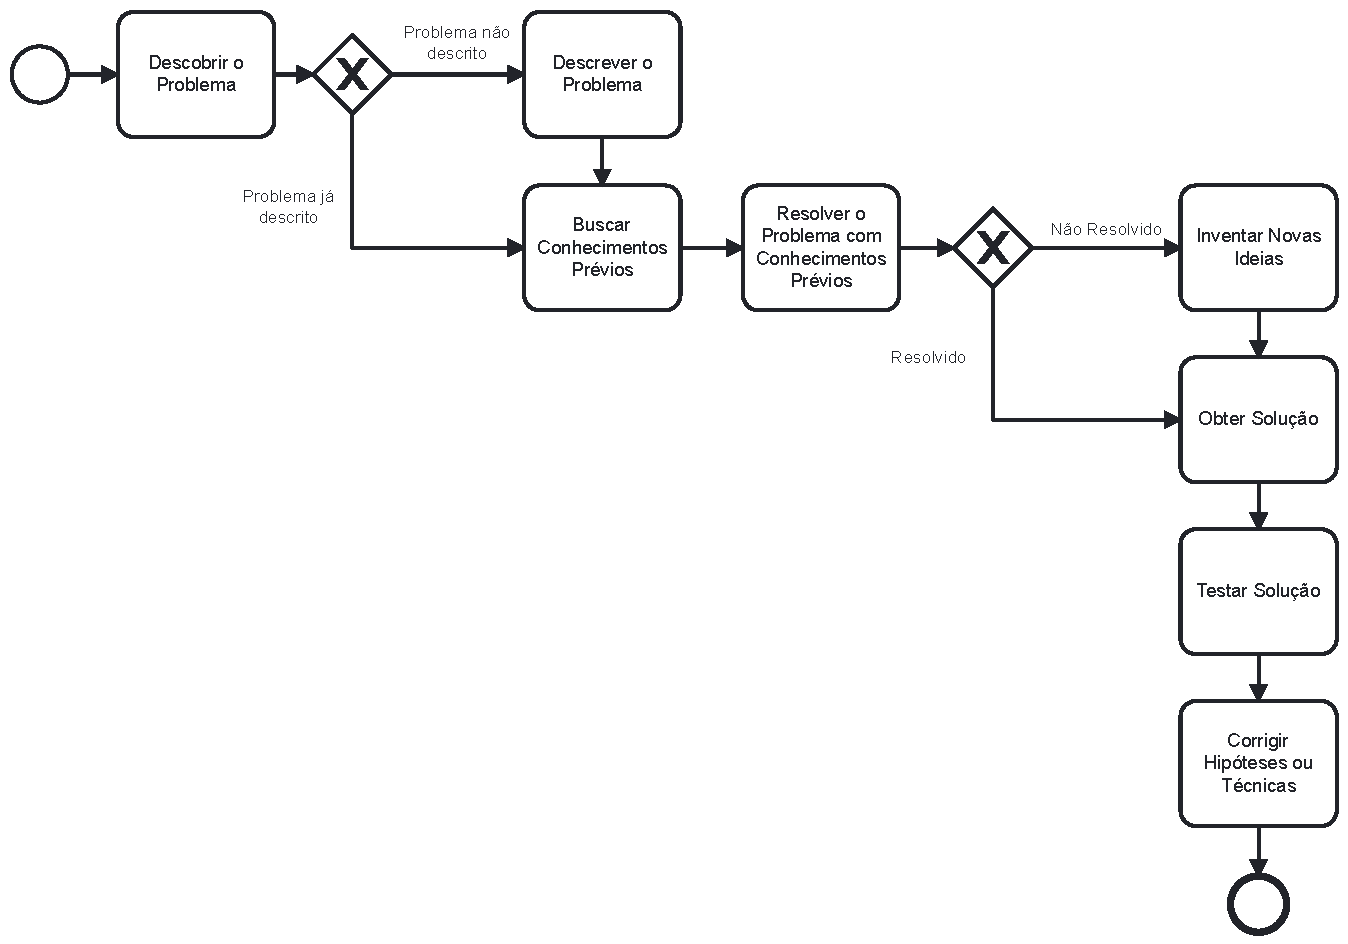
\includegraphics[width=0.7\linewidth]{Images/metodologiabunge.pdf}
    \caption{Metodologia Científica segundo \citet{Bunge2002}, descrita em BPMN~\citep{omg2013bpmn}. Fonte: Do Autor}
    \label{fig:bunge}
\end{figure}

O mesmo autor ainda diz que para que uma ideia seja considerada científica é necessário, mas não suficiente, que ela seja objetivamente testável com dados empíricos~\citep[p. 37]{Bunge2002}. 

Ainda mais, \citet[p. 40]{Bunge2002} cita \citet{Kuhn1970}, que diz que a melhor forma de aprender a planejar e resolver problemas científicos não é estudar um manual de metodologia, mas estudar e imitar paradigmas ou modelos de investigações que tiveram êxito. \citet{Kuhn2018}, em seu posfácio de 1969, cita outro autor, Michael Polanyi,  e defende o conhecimento tácito,  dizendo que ele ``é aprendido fazendo ciência, ao invés de adquirindo regras para fazê-la''~\citep[p. 160]{Kuhn2018}\footnote{O que é um sinal de aviso sobre este texto!}.

A escolha do método científico é complexa e depende de vários fatores do contexto a que o candidato está exposto. 

Escolhendo um método científico específico, por exemplo, uma variante da\textit{ Design Science Research}\citep{hevner2004design,Pimentel2019}, o candidato deve estar ciente das questões envolvidas, seguir o método e defendê-lo. Outros métodos mais gerais podem ser seguidos com menos compromisso.

Essa questão precisa ser discutida, e tratada entre orientador e orientado.

\section{Como Fazer Uma Tese}

O mercado está cheio de livros sobre ``Como fazer uma tese'' e ``Metodologia Científica''. A verdade é que esses livros pouco ajudarão você. A grande maioria é burocrata, ensinando quantos centímetros deve ter uma ficha e o formato de uma bibliografia. O problema não é realmente fazer isso certo, mas se organizar para fazer. 

Até pouco tempo não conhecia nenhum livro que realmente poderia sugerir, mas hoje conheço dois:
\begin{itemize}
    \item \fullcite{freitas2001}
    \item \fullcite{wazlawick2020}
\end{itemize}
	
Esqueça o famoso livro de Umberto Eco, ``Como Fazer uma Tese'', ele não é bom para teses de mestrado e doutorado, fala sobre uma ``tesi di laurea'', que é equivalente a um projeto final no Brasil. O livro tem muitos comentários que não se aplicam à engenharia, outras áreas técnicas, e ao Brasil. 

Uma das coisas mais importantes é estar em dia com a literatura da área. Isso significa que você tem que visitar pelo uma vez por mês cada site que possa ser útil para você, procurando publicações novas. Essa visita, hoje em dia, é virtual, normalmente por meio do Portal de Periódicos da CAPES mas nunca subestime a capacidade que temos de ter ideias folheando uma revista ou livro. 
Ou seja, não confie apenas na busca, mas também leia ou folheie as revistas científicas.

\gxatencao{Use o portal da Capes em http://www.periodicos.capes.gov.br/.}


\section{Propor e Comprovar}

Uma tese é uma proposta científica que avança o estado da arte. Ou seja, ao escrever sua tese você está se propondo a melhorar alguma coisa. Mas não basta apenas a sua opinião de que algo realmente melhorou: é necessário comprovar essa melhora.

Para isso é necessário construir um experimento (ou fazer uma observação). Esse experimento se torna cada vez mais essencial nas teses e a tendência atual é que um aluno não vai defender tese sem algum tipo de comprovação científica.

Basicamente existem duas formas de comprovar algo: quantitativamente ou qualitativamente. No primeiro caso, você terá números claros que indicam a melhoria. Por exemplo, após rodar várias vezes dois algoritmos, você conclui que um é duas vezes mais rápido do que o outro. Qualitativamente você faz a comparação em alguns casos, comparando-os de forma subjetiva.
Lembre-se do que falou Werner Von Braun:

\gxatencao{Um resultado de um teste vale um milhão de opiniões de especialistas.}

Não confie cegamente na Internet.  Utilize o senso crítico e analise a importância da referência que está usando. Revistas indexadas são importantes fontes, congressos também. Outra fonte boa de artigos, principalmente para se aprofundar em um tema, são os relatórios técnicos produzidos pelas universidades. 

A principal recomendação é sempre ler: Leia muito. Leia artigos sobre a teoria e sobre a aplicação. Leia revistas correlatas. Leia o jornal diariamente. Leia revistas de divulgação científica relacionadas ao seu trabalho. Leia revistas importantes nacionais e internacionais. A leitura é um hábito importante e deve ser desenvolvido constantemente. Leve todos os artigos interessantes para seu orientador ver. Se forem muito interessantes, leve uma cópia para deixar com ele. Desenvolva o hábito de trabalhar com seu orientador. 





\section{Classificação dos Métodos de Pesquisa}

Os métodos de pesquisa científica podem ser classificados segundo diferentes critérios, dependendo da natureza do problema, dos objetivos do estudo, do tipo de dado coletado e do papel do pesquisador. Embora não exista uma única taxonomia universalmente aceita, a literatura de metodologia aplicada à Computação apresenta algumas divisões amplamente utilizadas. 
A seguir, exploramos as principais formas de classificar os métodos científicos com foco em pesquisas em Ciência da Computação e áreas aplicadas como Engenharia de Software e Sistemas de Informação.

\subsection{Quantitativo vs. Qualitativo}

Quanto ao tipo de dados coletado e a forma de análise realizada, as pesquisas se dividem em quantitativas e qualitativas.

A distinção entre métodos quantitativos e qualitativos é uma das mais tradicionais na metodologia científica. Embora essa separação não seja absoluta — muitos estudos contemporâneos adotam abordagens mistas — ela é útil para indicar diferenças de ênfase na coleta e análise de dados.

\begin{itemize}
\item \textbf{Pesquisas Quantitativas} lidam com dados numéricos e mensuráveis. São orientadas por hipóteses previamente formuladas e visam testar teorias ou comparar alternativas usando métodos estatísticos. São típicas em experimentos controlados, \textit{benchmarks} de desempenho e avaliações empíricas de algoritmos.
\item \textbf{Pesquisas Qualitativas}, por outro lado, buscam compreender fenômenos complexos a partir da interpretação de dados não-numéricos (entrevistas, textos, observações). São úteis para explorar fenômenos emergentes, compreender o comportamento de usuários ou identificar padrões em práticas sociais e organizacionais. Em Computação, são comuns em estudos de usabilidade, etnografias digitais, análise de logs e pesquisa-ação.
\end{itemize}

Em Computação, especialmente em Engenharia de Software e Sistemas de Informação, é comum empregar métodos qualitativos para levantar hipóteses ou compreender o contexto, e métodos quantitativos para testá-las, seguindo um ciclo iterativo.

\subsection{Exploratória, Descritiva, Explicativa}

Outra divisão tradicional é pelo \textbf{objetivo da pesquisa}:

\begin{itemize}
\item \textbf{Pesquisa Exploratória}: visa proporcionar maior familiaridade com o problema, levantando hipóteses ou identificando variáveis relevantes. É comum no início de um estudo, especialmente quando se conhece pouco sobre o fenômeno.
\item \textbf{Pesquisa Descritiva}: tem como objetivo principal a descrição de características, comportamentos ou padrões. Pode assumir tanto formas quantitativas (como surveys) quanto qualitativas (como análises de logs ou entrevistas estruturadas).
\item \textbf{Pesquisa Explicativa}: busca entender as causas ou os mecanismos por trás dos fenômenos observados. Em geral, envolve a formulação e teste de hipóteses, com um forte componente de validação.
\end{itemize}

Essas categorias não são mutuamente exclusivas: uma pesquisa exploratória pode evoluir para descritiva e, posteriormente, explicativa.

subsection{Pesquisa Experimental vs. Pesquisa Não-Experimental}

Em Computação, distingue-se também entre:

\begin{itemize}
\item \textbf{Pesquisa Experimental}, quando o pesquisador manipula variáveis independentes e observa os efeitos em variáveis dependentes, normalmente em um ambiente controlado. Exemplos: comparação de desempenho de algoritmos, avaliação de interfaces com usuários, testes A/B.
\item \textbf{Pesquisa Quase-Experimental}, quando há alguma manipulação, mas sem total controle das variáveis externas (como em ambientes organizacionais reais).

\item \textbf{Pesquisa Não-Experimental}, que inclui métodos observacionais ou baseados em dados existentes, como logs, entrevistas, estudos de caso, etc.
\end{itemize}


\subsection{Teórico vs. Aplicado}

Outra distinção relevante é entre:

\begin{itemize}
\item \textbf{Pesquisa Teórica}, voltada à formulação, formalização e análise de modelos, algoritmos e sistemas conceituais. Envolve forte abstração e contribuições formais.
\item \textbf{Pesquisa Aplicada}, direcionada à resolução de problemas práticos com base em teorias existentes ou artefatos novos. É predominante nas dissertações profissionais e trabalhos de Engenharia de Software.
\end{itemize}

\subsection{Métodos Empíricos em Computação Aplicada}

A literatura recente em Engenharia de Software, Informática na Educação e Interação Humano-Computador enfatiza o uso de métodos empíricos com foco prático. 

Alguns dos métodos mais recorrentes incluem:

\begin{itemize}
\item \textbf{Estudo de Caso (Case Study)}: método qualitativo ou misto, que analisa profundamente um ou poucos objetos de estudo em seu contexto natural. Usado para entender fenômenos complexos, é comum em avaliações de ferramentas, processos e organizações.
\item \textbf{Relato de Experiência (Experience Report)}: descreve o uso de uma tecnologia, ferramenta ou método em um cenário prático. Pode ser útil para documentar lições aprendidas, mas deve seguir critérios de rigor para evitar viés anedótico.
\item \textbf{Pesquisa-Ação (Action Research)}: o pesquisador atua diretamente no ambiente estudado, intervindo para solucionar um problema real e, ao mesmo tempo, gerar conhecimento científico. É apropriado em contextos educacionais, organizacionais ou comunitários.
\item \textbf{Survey}: coleta de dados estruturada com questionários, geralmente com objetivos descritivos ou correlacionais. Amplamente utilizada para obter a percepção de usuários ou desenvolvedores sobre práticas ou tecnologias.
\item \textbf{Grounded Theory}: permite derivar teorias emergentes a partir da análise de dados qualitativos. É recomendada para explorar fenômenos ainda não estruturados teoricamente.
\item \textbf{Experimentos Controlados}: envolvem manipulação deliberada de variáveis e medição de impacto. São comuns em testes de algoritmos, desempenho de sistemas, ou avaliação de abordagens didáticas.
\item \textbf{Revisões Sistemáticas}: fundamentais para identificar lacunas no conhecimento e sintetizar o estado da arte, como também descrito anteriormente.
\end{itemize}

\section{Design Science Research}

A \textit{Design Science Research} (DSR) é uma ``abordagem que legitima o desenvolvimento de artefatos como um meio para produção de conhecimentos científicos''~\citep{Pimentel2019}. 

\citet{Pimentel2019} diz que o pesquisador ao usar a DSR se compromete com ``resolver um problema prático num contexto específico por meio de um artefato'' e ``gerar novo conhecimento científico''.

Seu uso, porém, implica em criar um modelo correto do trabalho a ser feito, incluindo descrições do problema, do artefato e conjecturas teóricas sobre o contexto onde o artefato será usado.

Apesar de atraente como metodologia de pesquisa, muitos dos trabalhos que tentam justificar sua metodologia por essa abordagem acabam por falhar, sendo bastante criticados, principalmente pela falta de uma formalização científica. É dado muito foco ao artefato, mas não a Ciência\citet{Pimentel2019}.

%O aluno pode tentar outras abordagens, partindo, por exemplo, diretamente da obra de \citet{Hevner2004}, ou ainda de \citet{Wieringa2014}. 

% Chamamos a atenção que uma pesquisa em DSR precisa, por sua natureza, de ciclos de proposta e avaliação, o que pode não caber no tempo destinado a uma dissertação de mestrado. 
% Além disso, o problema precisa ser avaliado em seu contexto, o que pode exigir um passo adicional aos experimentos.

\subsection{Como Usar a DSR}

A proposta aqui delineada busca estabelecer um modelo comum de trabalho para garantir coerência, rigor científico e alinhamento às melhores práticas internacionais na área, a partir da adoção da DSR. 

Este texto é um guia inicial para o uso do DSR e outros métodos associados, exigindo a leitura da documentação sobre os métodos.

Design Science Research (DSR) é uma abordagem metodológica que visa a construção e avaliação de artefatos para resolver problemas complexos no contexto das ciências aplicadas, como a Engenharia de Software, Sistemas de Informação e Ciência da Computação em geral~\citep{hevner2004design}. 

A DSR diferencia-se das abordagens tradicionais por focar não apenas na compreensão do fenômeno, mas na intervenção com base em um conhecimento científico rigoroso \cite{hevner2004design, peffers2007design}. Assim, ela busca contribuir tanto para a prática quanto para a teoria.

A minha orientação atual ao adotar a DSR é modelar o trabalho com o método MODEL-DSR~\citep{pimentel2019dsr,pimentel2023} e produzir os artefatos segundo o \textit{Framework de Pesquisa em Tecnologia da Informação}. Isso vem mudando ao longo do tempo, e isso é o que considero a melhor prática em 2025.


\subsection{Um Modelo de Pesquisa em DSR - MODEL-DSR}

O MODEL-DSR é uma proposta metodológica desenvolvida por Pimentel, Filippo e Santoro \cite{pimentel2019dsr,pimentel2023}, com o objetivo de orientar pesquisas em Informática na Educação a partir dos princípios da Design Science Research. 

Segundo \citet{pimentel2023} ``O modelo consiste em um conjunto de elementos que precisam estar coerentemente inter-relacionados''. Dado um problema que existe dentro de um contexto, um artefato é construído direcionado por conjecturas comportamentais. O artefato então permite a avaliação do problema em contexto e da conjectura (ver \autoref{fig:dsrmodel})

\begin{figure}
    \centering
    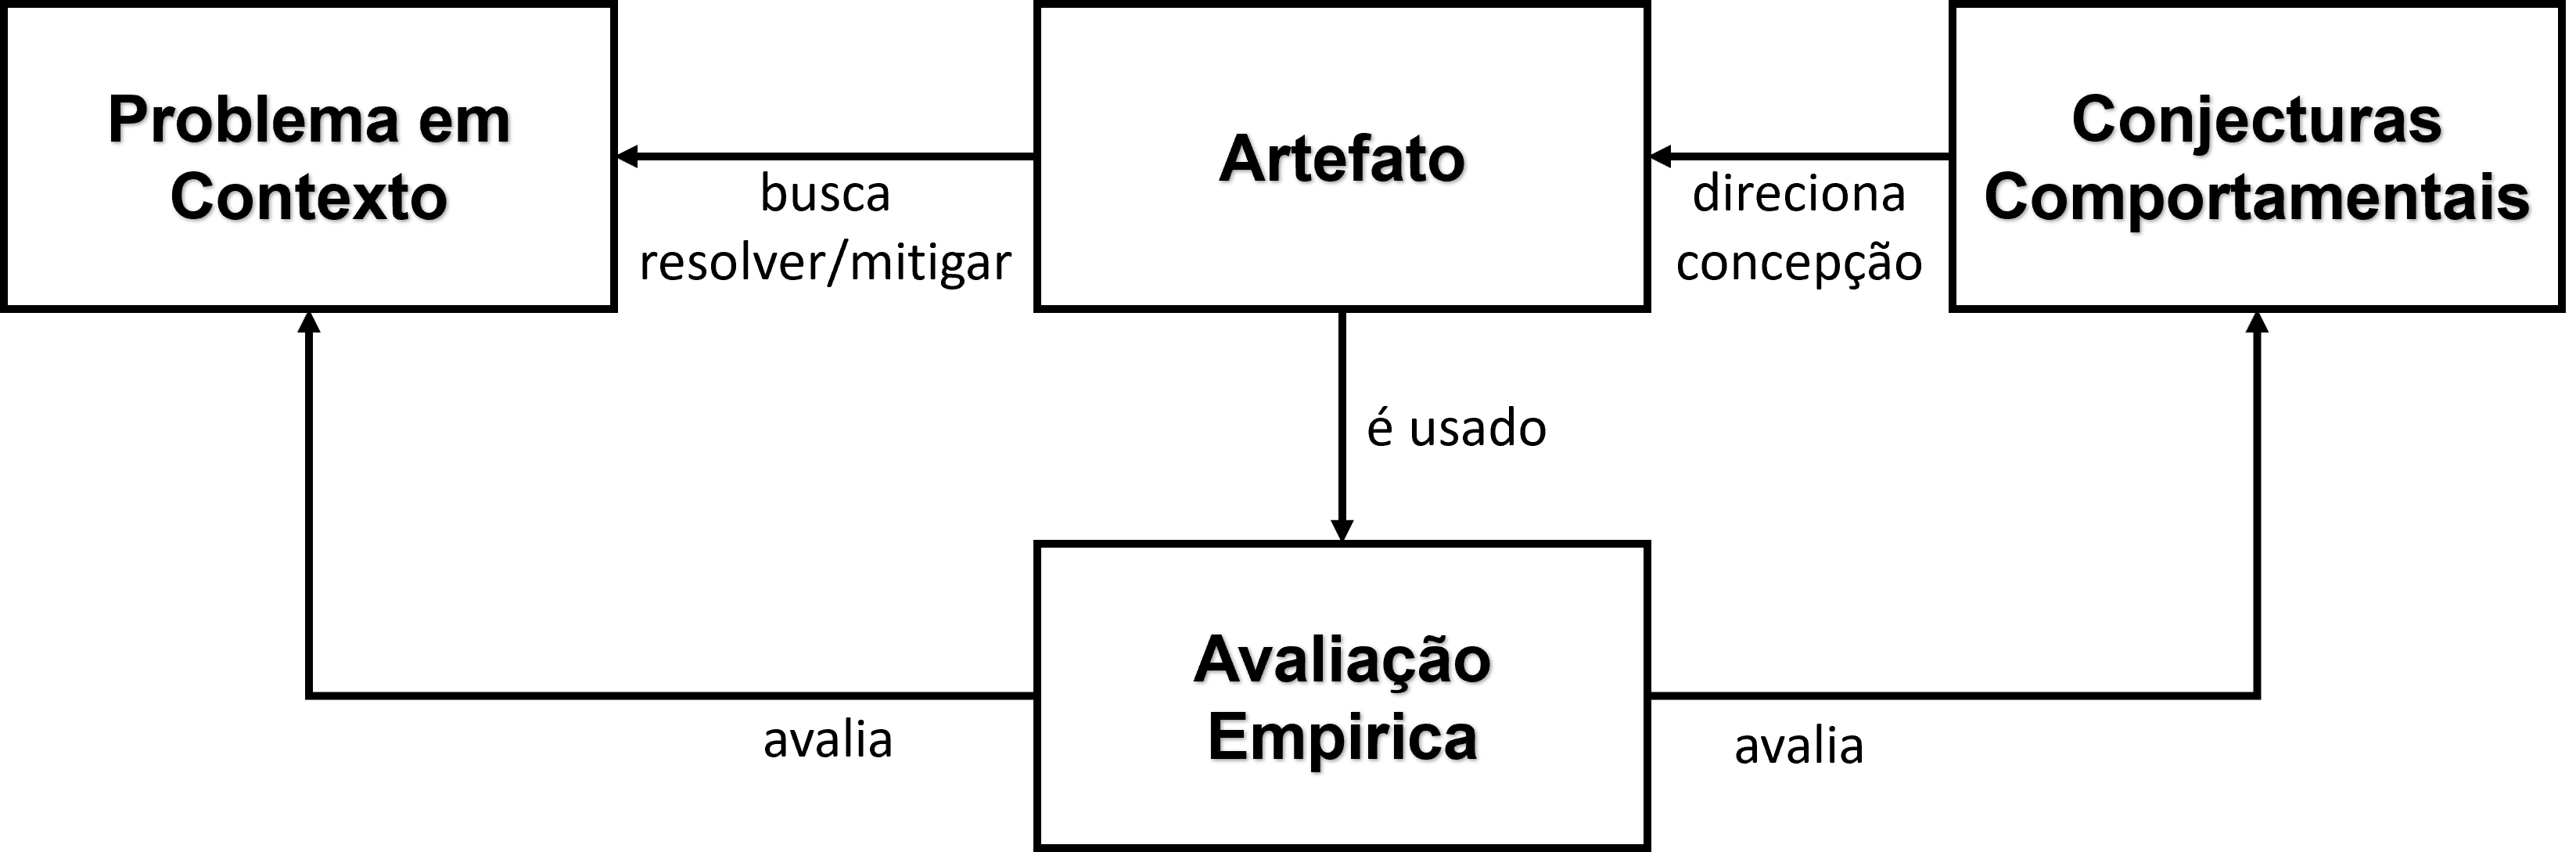
\includegraphics[width=0.5\linewidth]{Images/dsr pimental.png}
    \caption{Elementos centrais do Model-DSR. Baseado em \citep{pimentel2023}}
    \label{fig:dsrmodel}
\end{figure}

O modelo também propõe um artefato visual que explicita as conexões entre teoria, problema, solução e contexto. Esse artefato é adotado por nosso grupo para definir a pesquisa que está sendo feita. Exemplos foram dados por \citet{pimentel2019dsr} e \citet{pimentel2023}.

Ao destacar a produção de conhecimento científico como elemento central da DSR, o MODEL-DSR contribui para diferenciar claramente pesquisa de desenvolvimento tecnológico. Ele é especialmente adequado a pesquisas aplicadas em educação mediada por tecnologia, promovendo o rigor metodológico e a relevância prática.

\subsection{Framework de Pesquisa em Tecnologia da Informação}

March e Smith \cite{march1995design} propuseram um framework bidimensional (ver \autoref{tab:marchsmith}) para pesquisas em Tecnologia da Informação que distingue entre tipos de artefatos produzidos e atividades de pesquisa realizadas. Os artefatos incluem:
\begin{itemize}
    \item \textbf{Construtos}: são os conceitos que formam a linguagem da área de estudo, usados para descrever problemas e formular soluções.
    \item \textbf{Modelos}: expressam relações entre construtos e servem como representacões de situações-problema ou de soluções.
    \item \textbf{Métodos}: são sequências de passos ou algoritmos utilizados para resolver tarefas específicas.
    \item \textbf{Instâncias}: são realizações concretas de sistemas, ferramentas ou protótipos que demonstram o uso prático dos construtos, modelos e métodos.
\end{itemize}

As atividades de pesquisa compreendem:
\begin{itemize}
    \item \textbf{Construção (build)}: desenvolvimento dos artefatos para um objetivo específico, demonstrando sua viabilidade.
    \item \textbf{Avaliação (evaluate)}: análise sistemática do desempenho dos artefatos em função de métricas e critérios estabelecidos.
    \item \textbf{Teorização (theorize)}: construção de explicações que descrevem como e por que os artefatos funcionam em seu ambiente.
    \item \textbf{Justificativa (justify)}: verificação empírica ou formal das teorias propostas, com base em evidências.
\end{itemize}

Esse framework contribui para organizar e avaliar as pesquisas em TI segundo seu tipo de contribuição, facilitando a compreensão e a comunicação dos resultados científicos.

\begin{table}[hbt]
    \centering
    \begin{tabular}{|c|c|c|c|c|}
    \hline
       & Construção & Avaliação & Teorização & Justificativa  \\    \hline
    Construtos &&&&\\     \hline
    Modelo &&&&\\    \hline
    Método &&&&\\    \hline
    Instâncias &&&&\\    \hline
    \end{tabular}
    \caption{O \textit{Framework} de pesquisa em tecnologia da informação proposto por \citet{march1995design}}
    \label{tab:marchsmith}
\end{table}

Além disso, Hevner et al. \cite{hevner2004design} destacam que a contribuição para o corpo de conhecimento científico é um critério essencial para a validade de uma pesquisa baseada em DSR.

\subsection{Como Não Usar  DSR}

A DSR não é uma solução mágica, principalmente não é uma resposta para ser dada no final de uma tese feita por tentativa e erro. 

O principal problema metodológico é o \textit{retrofit}. O candidato, que foi tateando em busca de uma solução para um problema que o agradava, e acabou por esquecer a metodologia, acaba tentando explicar o que fez com uma DSR ``mais ou menos''.

Claro que há uma culpa do orientador, porém quero lembrar que não só o único responsável pela tese é o orientado, como ele é o único que sofre consequências graves pelo seu erro.



\section{A Revisão Bibliográfica}


São dois os objetivos da revisão bibliográfica:
\begin{itemize}
    \item primeiro, ela deve comprovar que o futuro mestre cumpriu bem as fases iniciais da metodologia científica, isso é, o descobrimento e a descrição do problema e a busca de conhecimentos ou instrumentos relevantes ao problema;
    \item realizado isso, ela deve contextualizar o leitor no domínio do conhecimento. 
\end{itemize}

Uma dissertação de mestrado, porém, não é um documento fechado, que tudo explica, mas sim uma revisão dos conceitos do problema e da solução, e um guia para leituras mais detalhadas. 
Elas são similares a artigos de \textit{survey} e deviam, na prática, ser dignas de publicação como tal.

Seus leitores são de dois tipos principais: a banca, que tem alta especialização, e outros pesquisadores que podem buscar a dissertação como referência e modelo de como fazer o trabalho.

A revisão bibliográfica deve ser focada e deve tentar evitar discutir profundamente assuntos não diretamente correlacionados a dissertação.
É importante que a revisão sirva como um guia de leitura dos assuntos, comentado e fazendo ponderações em relação aos documentos citadas.

É costume separar a divisão, possivelmente em dois capítulos, entre a revisão do problema e a revisão das técnicas usadas na dissertação. A abordagem, em geral, é \textit{top-down}, fazendo uma descrição do mais geral ao mais específico.

Na prática, ela não deve ser uma lista de quem disse o quê, mas uma \textbf{revisão global e comparativa do conhecimento}, inclusive com uma visão histórica, e das relações entre aos problemas e propostas analisados.

Nas dissertações onde se resolve um problema específico, esse problema deve ser bem analisado e explicado, e, possivelmente, bem definido, caso não seja definido de forma apropriada na literatura, atendendo ao passo 2 do método científico. 

Finalmente, uma dos objetivos importantes da revisão bibliográfica é fazer uma análise da contribuição de cada texto revisto, de modo a poder contextualizar a contribuição apresentada na dissertação.


\subsection{Revisões Sistemáticas}

Revisões sistemáticas são ferramentas essenciais para a identificação de lacunas no conhecimento e para fundamentar a construção de artefatos na DSR. Kitchenham et al. \cite{kitchenham2004procedures} definem revisões sistemáticas como um processo rigoroso, transparente e reprodutível de seleção e análise de literatura.

Existem vários modelos similares com objetivos semelhantes, que 

A integração de revisões sistemáticas, ou similares, à DSR assegura que a pesquisa se apoie em uma base sólida de conhecimento existente, aumentando sua relevância e contribuição científica.

Para escolher uma forma de revisão, o artigo de \citet{grant2009typology} lista 14 tipos. A partir daí é necessário buscar a descrição da forma mais adequada de fazê-lo. A Linha de Engenharia de Software trabalha há algum tempo com revisões sistematizadas e é possível encontrar não só definições de como devem ser feitas, mas também bons exemplos entre as teses, dissertações e relatórios técnicos do PESC~\footnote{\url{https://cos.ufrj.br/index.php/pt-BR/publicacoes-pesquisa}}


\section{Outros Métodos Recomendados}


\subsection{Grounded Theory}

Grounded Theory (GT) é uma metodologia qualitativa que busca desenvolver teorias a partir de dados empíricos coletados sistematicamente. Proposta originalmente por Glaser e Strauss \cite{glaser1967discovery}, ela é particularmente útil para explorar áreas onde as teorias ainda estão em formação. 
No contexto da DSR, a GT pode ser utilizada para identificar problemas relevantes ou avaliar a implementação de artefatos, contribuindo assim para o rigor teórico da pesquisa.

Em especial no nosso caso, essa teoria pode ser usada para elicitar Construtos, Modelos e Métodos.

